% This is LLNCS.DEM the demonstration file of
% the LaTeX macro package from Springer-Verlag
% for Lecture Notes in Computer Science,
% version 2.4 for LaTeX2e as of 16. April 2010
%
\documentclass[runningheads]{llncs}
\usepackage{graphicx}
%\usepackage{bm}
%\usepackage{url}
\usepackage{epstopdf}
\usepackage{url}
\usepackage[usenames]{xcolor}
\usepackage[vlined]{algorithm2e}
\usepackage{multirow}
\usepackage{rotating}

\newcommand{\Jose}[1]{{\color{red} [[JOSE:: #1]]}}
\newcommand{\Leo}[1]{{\color{blue} [[LEO:: #1]]}}
\newcommand{\Meng}[1]{{\color{green} [[MENG:: #1]]}}
\newcommand{\Norbert}[1]{{\color{orange} [[NORBERT:: #1]]}}
 
\usepackage{amsmath}
\usepackage{amssymb}
%* Commands and Environments:  %%%%%%%%%%%%%%%%%%%%%%%%%%%%%%%%%%%%%%%%
%** Macros from JeffreyScottVitter
% Write multichar identifier names using \id in either mathmode or text;
% For ex, $\id{high}(x)$ is an expression using the \id{high} function.
% Use ``\ '' if a space is desired, as in math mode.
\def\id#1{\ensuremath{\mathit{#1}}}
\let\idit=\id
\def\idbf#1{\ensuremath{\mathbf{#1}}}
\def\idrm#1{\ensuremath{\mathrm{#1}}}
\def\idtt#1{\ensuremath{\mathtt{#1}}}
\def\idsf#1{\ensuremath{\mathsf{#1}}}
\def\idcal#1{\ensuremath{\mathcal{#1}}}  % Use with capital letter args only


\def\poly{\idtt{poly}}

\def\access{\idtt{access}}
\def\findopen{\idtt{find\_open}}
\def\findclose{\idtt{find\_close}}
\def\enclose{\idtt{enclose}}
\def\selectopen{\idtt{select\_open}}
\def\selectclose{\idtt{select\_close}}
\def\rankopen{\idtt{rank\_open}}
\def\rankclose{\idtt{rank\_close}}
\def\rmqi{\idtt{rmqi}}
\def\RMQi{\idtt{RMQi}}
\def\child{\idtt{child}}
\def\childrank{\idtt{child\_rank}}
\def\depth{\idtt{depth}}
\def\levelanc{\idtt{level\_anc}}
\def\subtreesize{\idtt{subtree\_size}}
\def\degree{\idtt{degree}}
\def\height{\idtt{height}}
\def\deepestnode{\idtt{deepest\_node}}
\def\lca{\idtt{LCA}}
\def\lmostleaf{\idtt{lmost\_leaf}}
\def\rmostleaf{\idtt{rmost\_leaf}}
\def\leafrank{\idtt{leaf\_rank}}
\def\leafselect{\idtt{leaf\_select}}
\def\prerank{\idtt{pre\_rank}}
\def\postrank{\idtt{post\_select}}
\def\preselect{\idtt{pre\_select}}
\def\postselect{\idtt{post\_select}}
\def\nodeselect{\idtt{node\_select}}
\def\levellmost{\idtt{level\_lmost}}
\def\levelrmost{\idtt{level\_rmost}}
\def\levelsucc{\idtt{level\_succ}}
\def\levelpred{\idtt{level\_pred}}
\def\sumop{\idtt{sum}}
\def\fwdsearch{\idtt{fwd\_search}}
\def\bwdsearch{\idtt{bwd\_search}}
\def\rmq{\idtt{rmq}}
\def\RMQ{\idtt{RMQ}}


\def\rankop{\idtt{rank}}
\def\selop{\idtt{select}}

\newenvironment{myitemize}%
  {\begin{itemize}%
    \setlength{\itemindent}{-.1in}
    \setlength{\itemsep}{\baselineskip}%
    \setlength{\parskip}{-\baselineskip}}%
  {\end{itemize}}

\DeclareMathOperator*{\argmin}{arg\!\min}
\DeclareMathOperator*{\argmax}{arg\!\max}
%\newtheorem{lemma}{Lemma}



\begin{document}


\title{Parallel Construction of Succinct Trees\thanks{This work was supported in part by Jos\'e Fuentes-Sepúlveda's scholarship, granted by Government of Canada.}}
\titlerunning{Parallel Construction of Succinct Trees}

\author{Leo Ferres\inst{1} \and Jos\'e Fuentes-Sep\'ulveda\inst{1} \and Meng He\inst{2} \and Norbert Zeh\inst{2}}

\authorrunning{Leo Ferres, Jos\'e Fuentes-Sep\'ulveda, Meng He, and Norbert Zeh} % abbreviated author list (for running head)
%
%%%% list of authors for the TOC (use if author list has to be modified)
\tocauthor{Leo Ferres, Jos\'e Fuentes-Sep\'ulveda, Meng He, and Norbert Zeh}
%
\institute{Department of Computer Science, Universidad de Concepci\'on, Chile,\\
\email{\{lferres,jfuentess\}@udec.cl},
\and
Faculty of Computer Science, Dalhousie University, Canada,\\
\email{\{mhe,nzeh\}@cs.dal.ca}}
  

\maketitle              % typeset the title of the contribution

\begin{abstract}
Succinct representations of trees have been an elegant solution to make large trees fit in main memory while still supporting
navigational operations in constant time. However, the construction time of succinct trees remains a computational bottleneck. In this
paper, we introduce a practical parallel algorithm that improves the state-of-the-art in succinct tree construction. Given a tree on
$n$ nodes stored as a sequence of balanced parentheses, the proposed algorithm can build a succinct tree representation in
$O(n/p+\lg p)$ time, where $p$ is the number of available processors. The constructed representation occupies $2n + o(n)$
bits of storage and supports a rich set of navigational operations in $O(\lg n)$ time. We tested the algorithm on a $64$-core
machine and on inputs of different sizes.
In these experiments, it achieved good parallel speedup.
Besides, since the succinct tree representation considered in our work is built upon the balanced parenthesis representation of the given
tree, we also introduce an algorithm to compute this parenthesis representation in $O(n/p+\lg p)$ time.
\end{abstract}
%

%%%%%%%%%%%%%%%%%%%%%%%%
%%%%% INTRODUCTION %%%%%
%%%%%%%%%%%%%%%%%%%%%%%%

\section{Introduction}
\label{sec:introduction}
Trees are ubiquitous in Computer Science.  They have applications in
every aspect of computing from XML/HTML processing to abstract syntax
trees (AST) in compilers, phylogenetic trees in computational genomics
or shortest path trees in path planning.  The ever increasing amounts
of structured, hierarchical data processed in many applications have
turned the processing of the corresponding large tree structures into
a bottleneck, particularly when they do not fit in memory.  Succinct
tree representations store trees using as few bits as possible and
thereby significantly increase the size of trees that fit in memory
while still supporting important primitive operations in constant
time.  There exist such representations that use only $2n - \Theta(\lg
n)$ bits\footnote{We use $\lg x$ to mean $\log_{2}x$ throughout this
paper.} to store the topology of a tree with $n$ nodes, which is close
to the information-theoretic lower bound and much less than the space
used by traditional pointer-based representations.

Alas, the construction of succinct trees is quite slow compared to the
construction of pointer-based representations.  Multicore parallelism
offers one possible tool to speed up the construction of succinct
trees, but little work has been done in this direction so far.  The
only results we are aware of focus on the construction of Wavelet
trees, which are used in representations of text indexes.  In
\cite{Fuentes2014}, two practical multicore algorithms for Wavelet
tree construction were introduced.  Both algorithms perform $O(n\lg
\sigma)$ work and have span $O(n)$, where $n$ is the input size and
$\sigma$ is the alphabet size.  In \cite{DBLP:journals/corr/Shun14},
Shun introduced three new algorithms to construct Wavelet trees in
parallel.  The in practice best algorithm performs $O(n\lg \sigma)$
work and has span $O(\lg n\lg \sigma)$.  Shun also explained how to
parallelize the construction of rank/select structures so it requires
$O(n)$ work and $O(1)$ span for rank structures, and $O(n)$ work and
$O(\lg n)$ span for select structures.

In this paper, we provide a parallel algorithm that constructs the
{\tt RMMT} tree representation of
\cite{Navarro:2014:FFS:2620785.2601073} in $O(n/p + \lg p)$ time
using $p$ cores.  This structure uses $2n + o(n)$ bits to store an
ordinal tree with $n$ nodes and supports a rich set of basic
operations on these trees in $O(\lg n)$ time.  While this query time
is theoretically suboptimal, the {\tt RMMT} structure is simple enough
to be practical and has been verified experimentally to be very small
and support fast queries in practice~\cite{ACNSalenex10}.  Combined
with the fast parallel construction algorithm presented in this paper,
it provides an excellent tool for manipulating very large trees in
many applications.

We implemented and tested our algorithm on a number of real-world input trees
having billions of nodes.
Our experiments show that our algorithm run on a single core is competitive with
state-of-the-art sequential constructions of the {\tt RMMT} structure and
achieves good speed-up on up to 64 cores and likely beyond.

\ignore{The remainder of this paper is organized as follows:
Section~\ref{sec:relwork} gives a brief overview of the {\tt RMMT}
structure, to clearly define its structure and illustrate how it can
be used to support basic operations on trees efficiently.  It also
briefly discusses other previous work on succinct tree representations
and reviews the dynamic multithreading model, which we use to analyze
the theoretical running time of our algorithm.
Section~\ref{sec:multicoreST} describes our parallel algorithm for
constructing the {\tt RMMT} structure.  Section~\ref{sec:exps}
discusses our experimental setup and results.
Section~\ref{sec:conclusion} offers concluding remarks and discusses
future work.}

%%% Local Variables:
%%% mode: plain-tex
%%% TeX-master: t
%%% End:



%%%%%%%%%%%%%%%%%%%%%%%%
%%%%% PRELIMINARIES %%%%%
%%%%%%%%%%%%%%%%%%%%%%%%

\section{Preliminaries}
\label{sec:relwork}
\Jose{Here we should introduce the Range Min-Max Tree}

\subsection{Succinct Trees}
\label{subsec:suctrees}
Jacobson~\cite{j1989} first proposed to design succinct data structures.
He showed how to represent an ordinal trees on $n$ nodes using $2n+o(n)$ bits so
that computing the first child, the next sibling or the parent of any given node
takes $O(\lg n)$ time in the bit probe model.
Clark and Munro~\cite{cm1996} showed how to support the same operations in
constant time in the word RAM model with word size $\Theta(\lg n)$.
Since then, a lot of work has been done on succinct tree representations, to
support more navigational operations, to achieve compression, to provide support
for update operations, and so
on~\cite{mr1997,bdmr1999,grr2004,jss2007,ly2008,hms2012,fm2014,Navarro:2014:FFS:2620785.2601073}. 
Raman and Rao~\cite{rr2013} give a thorough survey of the state of the art.

In this paper, we present a parallel algorithm to construct the succinct tree
representation proposed recently by Navarro and
Sadakane~\cite{Navarro:2014:FFS:2620785.2601073}, referred to as
NS-representation throughout this paper.
This representation is the first to achieve a {\em redundancy}
of $O(n/\lg^c n)$ bits for any positive constant $c$.
The redundancy is the additional space used by the data structure above the
information-theoretic lower bound.
While all previous tree representations achieved a redundancy of $o(n)$ bits,
their redundancy was $\Omega(n \lg\lg n / \lg n)$ bits, that is, just slightly
sub-linear.
The NS-representation also supports a large number of
navigational operations in constant time (see Table~\ref{tbl:operations}); only
the work in \cite{hms2012,fm2014} supports two more operations.
The main reason we focus on this representation in this paper is an experimental
study on succinct trees~\cite{ACNSalenex10}, which showed that an implementation
of a simplified version ofthe NS-representation uses less space than other
existing representations in most cases and performs most operations faster.
Our goal in this paper is to alleviate the construction bottleneck of this
representation by exploiting multicore parallelism.

\begin{table}[t]
\begin{center}
\begin{tabular}{|>{\raggedright}p{2.4cm}|>{\raggedright\arraybackslash}p{5.2cm}|} \hline
\bf Operation                         & \bf Description        \\ \hline
$\child(x,i)$                         & Report $i$th child of node $x$\\
$\childrank(x)$                       & Report number of left siblings of node $x$\\
$\degree(x)$                          & Report degree of node $x$\\
$\depth(x)$                           & Report depth of node $x$\\
$\levelanc(x,i)$                      & Find ancestor of node $x$ that is $i $levels above node $x$ \\
$\subtreesize(x)$                     & Report number of nodes in the subtree rooted at node $x$ \\
$\height(x)$                          & Report height of the subtree rooted at $x$ \\
$\deepestnode(x)$                     & Find deepest node in the subtree rooted at node $x$\\
$\lca(x,y)$                           & Find lowest common ancestor of nodes $x$ and $y$ \\
$\lmostleaf(x)$ /$\rmostleaf(x)$      & Find leftmost/rightmost leaf of the subtree rooted at node $x$\\
$\leafrank(x)$                        & Report Number of leaves before node $x$ in preorder\\
$\leafselect(i)$                      & Find $i$th leaf from left to right\\
$\prerank(x)$ /$\postrank(x)$         & Report number of nodes preceding node $x$ in preorder/postorder\\
$\preselect$ /$\postselect(i)$        & Find $i$th node in preorder/postorder\\       
$\levellmost(i)$ /$\levelrmost(i)$    & Find leftmost/rightmost node among all the nodes at depth $i$ \\
$\levelsucc(x)$ /$\levelpred(x)$      & Find node immediately to the left/right of node $x$ among nodes at the same depth\\ \hline
$\access(i)$                          & Report the $i$th parenthesis $P[i]$        \\ 
$\findopen(i)$ /$\findclose(i)$       & Find the matching parenthesis of $P[i]$ \\
$\enclose(i)$                         & Find the closest enclosing matching parenthesis pair for $P[i]$ \\
$\rankopen(i)$ /$\rankclose(i)$       & Report the number of opening/closing parentheses in $P[1..i]$\\
$\selectopen(i)$ /$\selectclose(i)$   & Find the $i$th opening/closing parenthesis\\ \hline
\end{tabular}
\caption{Operations supported by the NS-representation, including operations
  on the corresponding balanced parenthesis sequence.}
\label{tbl:operations}
\end{center}
\end{table}

The NS-representation is based on the balanced parenthesis sequence $P$ of
the input tree, which is obtained by performing a preorder traversal
of the given tree and writing down an opening parenthesis when visiting
a node for the first time and a closing parenthesis after visiting
all its descendants.
Thus, the length of $P$ is $2n$.
The parenthesis sequence of the ordinal tree in Figure~\ref{figure:bp}, for
example, is $P = ((())((()())(()(())))()())$.

\begin{figure}
  \centering
  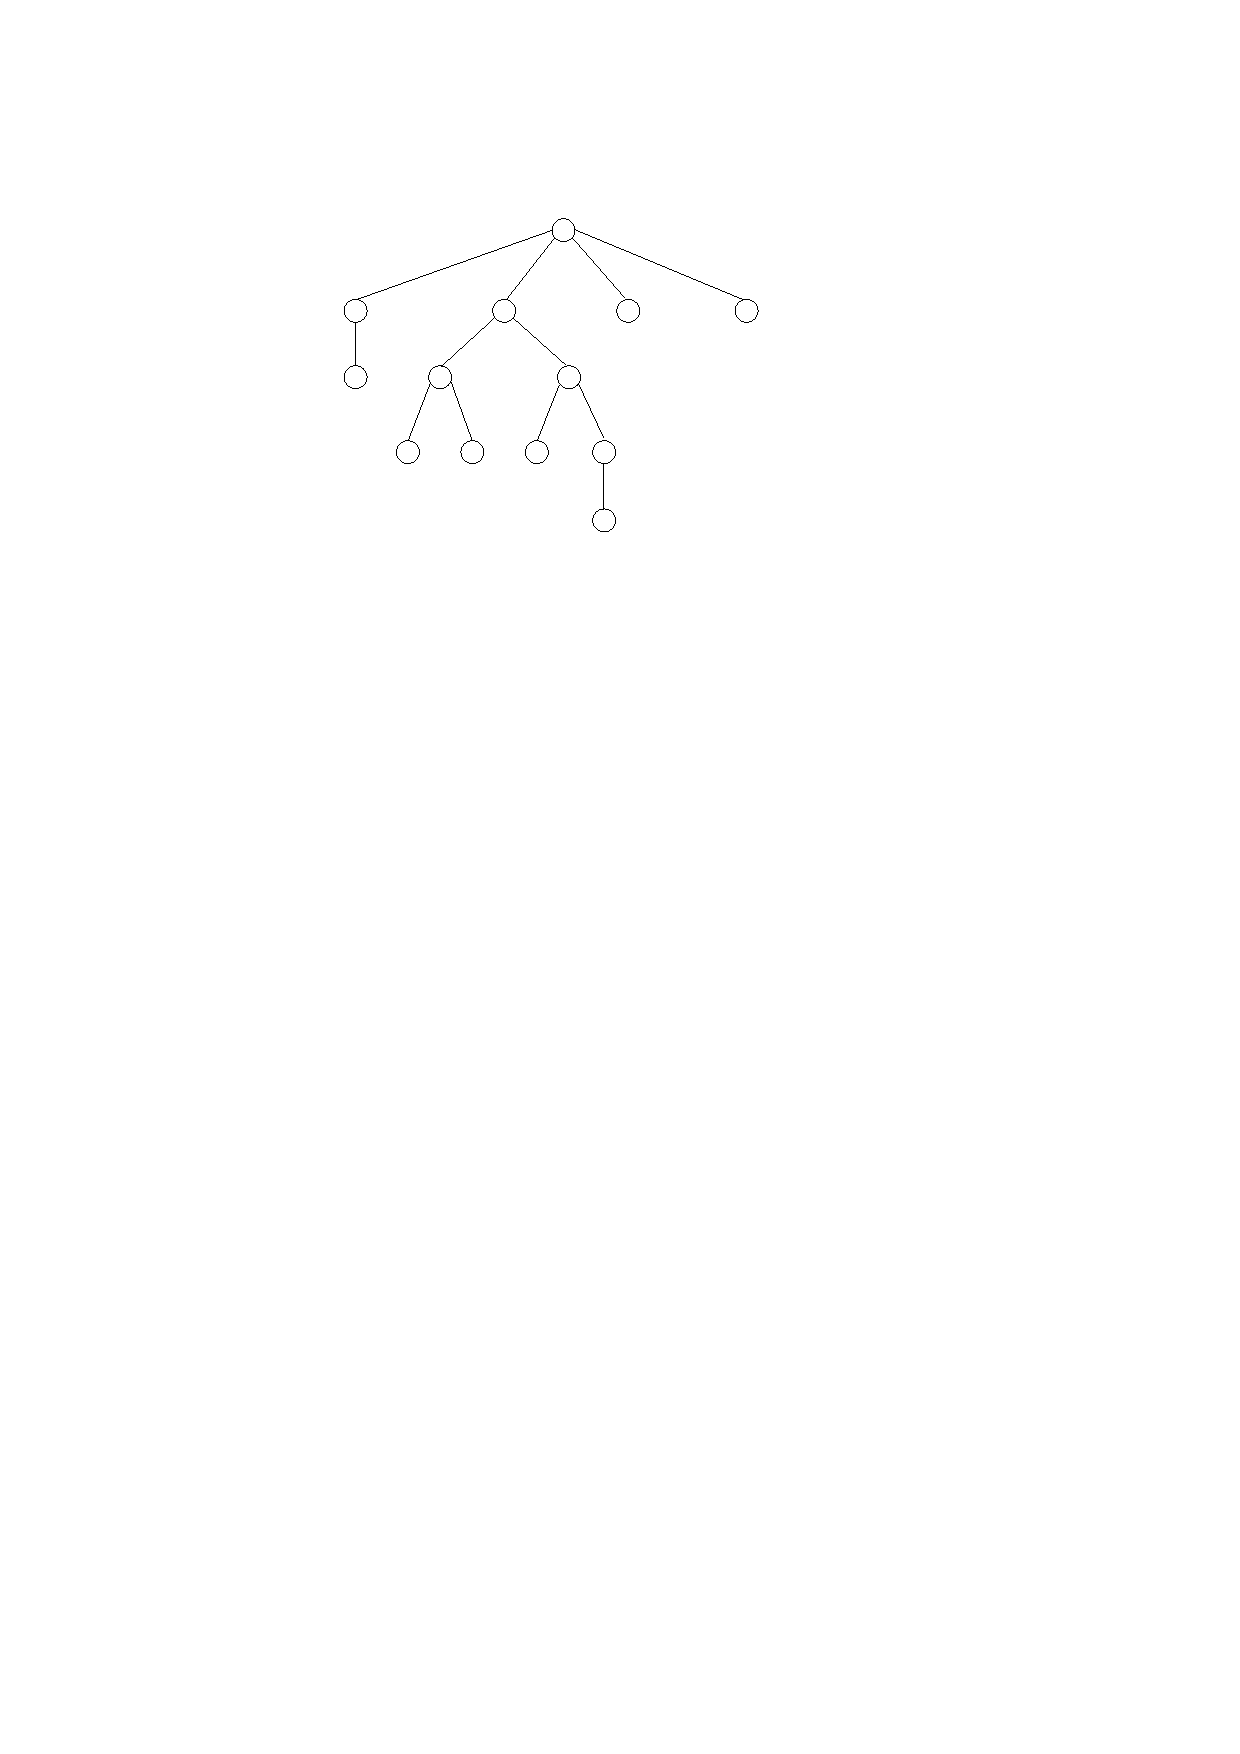
\includegraphics[scale=0.5]{images/bp.pdf}
  \caption{An ordinal tree used as an example.}
  \label{figure:bp}
\end{figure}

The NS-representation is not the first structure to use balanced parentheses to
represent trees.
Munro and Raman~\cite{mr1997} were the first to design succinct representations
of balanced parentheses and used them to represent ordinal trees succinctly by
reducing a set of navigational operations on trees to operations on their
balanced parenthesis sequences.
Their solution supports only a subset of the operations listed in
Table~\ref{tbl:operations}.
Additional operations can be supported using  auxiliary data
structures~\cite{ly2008}.
To support all operations in Table~\ref{tbl:operations}, many auxiliary data
structures are required, which add to the size of the final data structure
and make it complex in both theory and practice.
The main novelty of Navarro and Sadakane's
work~\cite{Navarro:2014:FFS:2620785.2601073} lies in the strategy they used to
reduce a large set of operations on trees and balanced parenthesis sequences to
a small set of \emph{primitive operations}.
Representing $P$ as a bit vector storing a $1$ for each opening parenthesis
and a $0$ for each closing parenthesis, these primitive operations are the
following.
Here, $g$ is an arbitrary function on $\{0,1\}$.
\begin{align*}
\sumop(P,g,i,j) &= \textstyle\sum_{k=i}^jg(P[k])\\
\fwdsearch(P,g,i,d) &= \min\{j \mid j \ge i, \sumop(P,g,i,j) = d\}\\
\bwdsearch(P,g,i,d) &= \max\{j \mid j \le i, \sumop(P,g,j,i) = d\}\\
\rmq(P,g,i,j) &= \min\{\sumop(P,g,i,k) \mid i\le k\le j\}\\
\RMQ(P,g,i,j) &= \max\{\sumop(P,g,i,k) \mid i\le k\le j\}\\
\rmqi(P,g,i,j) &= \argmin_{k\in[i,j]}\{\sumop(P,g,i,k)\}\\
\RMQi(P,g,i,j) &= \argmax_{k\in[i,j]}\{\sumop(P,g,i,k)\}
\end{align*}
Navarro and Sadakane defined three functions on $[0,1]$:
\begin{align*}
  \pi  &: 1 \mapsto 1\quad 0 \mapsto -1\\
  \phi &: 1 \mapsto 1\quad 0 \mapsto 0\\
  \psi &: 1 \mapsto 0\quad 0 \mapsto 1
\end{align*}
Most of the operations in Table~\ref{tbl:operations} can then be supported using
the primitive operations by setting $g$ to be $\pi$, $\phi$ or~$\psi$.
For example, $\findclose(i) = \fwdsearch(P,\pi,i,0)$.
Thus, it suffices to support the operations in Table~\ref{tbl:operations} for
$g = \pi$, $g = \phi$ or $g = \psi$, as well as a few navigational operations
that cannot expressed using these primitive operations, which are $\degree$,
$\child$, $\childrank$ and the four operations in Table~\ref{tbl:operations}
related to leaf nodes.
To support the primitive operations, Navarro and Sadakane designed a simple data
structure called \emph{Range Min-Max Tree} ({\tt RMMT}) (see next subsection).
It supports the primitive operations in logarithmic time when used to represent
the entire sequence~$P$.
To achieve constant-time operations, $P$ is further partitioned into chunks.
Each chunk is represented using a {\tt RMMT}, which can support primitive
operations inside the chunk in constant time if the chunk is small enough.
Additional data structures are used to support operations on the entire sequence
$P$ in constant time.

\subsubsection{The Range Min-Max Tree}

Let $w$ denote the number of bits in a word.
The range min-max tree ({\tt RMMT}) is designed to support the primitive
operations for functions $\pi$, $\phi$, and $\psi$.
We first describe how to construct a {\tt RMMT} for the function $\pi$ and
later show how it can be easily augmented to support the primitive operations
for the other two functions.
Recall that $T$ denotes the input tree on $n$ nodes, and $P$ represents its
balanced parenthesis sequence, where $P[i] = 1$ iff the $i$th
parenthesis is an opening parenthesis.
To define the {\tt RMMT}, we partition $P[1..2n]$ into disjoint chunks of
a size $s \le w/2$ to be chosen later.
For simplicity, we assume that the length of $P$ is a multiple of~$s$.
The {\tt RMMT} is a complete $k$-ary tree over the sequence of these chunks,
for some \emph{arity} $k \ge 2$ to be chosen later (see
Figure~\ref{fig:RangeMinMaxTree}).

Next define the following five arrays $E$, $e$, $m$, $M$, and $n^*$.
These arrays are only used in the description and are not stored explicitly
in the data structure.
The {\em excess} at position $i$ of $P$ is defined as $\sumop(P,\pi,0,i) =
\sum_{k=0}^{i} \pi(P[k])$.
$E$ has length $2n$ and $E[i]$ is the excess at position $i$.
The other four arrays are of length $2n/s$ each.
$e[i]$ stores the excess at position $is$, that is, at the end of the $i$th
chunk.
$m[i]$ and $M[i]$ store the minimum and maximum excess at any position in the
$i$th chunk, respectively.
$n^*[i]$ stores the number of positions in the $i$th chunk that have the
minimum excess value $m[i]$.
Each internal node, $u$, of the {\tt RMMT} also stores four similar values
$e[u]$, $m[u]$, $M[u]$, and $n^*[u]$, which have the same meaning as defined
above with respect to the subsequence of $P$ that is the concatenation of the
chunks corresponding to descendant leaves of $u$.
These values are illustrated in Figure~\ref{fig:RangeMinMaxTree}.
As the {\tt RMMT} is a complete tree, we do not store its structure explicitly.
Instead, we can simply store the values associated with its nodes in four arrays
$e'$, $m'$, $M'$, and $n'$ indexed like a $k$-ary heap.

\begin{figure}[t]
  \centering
  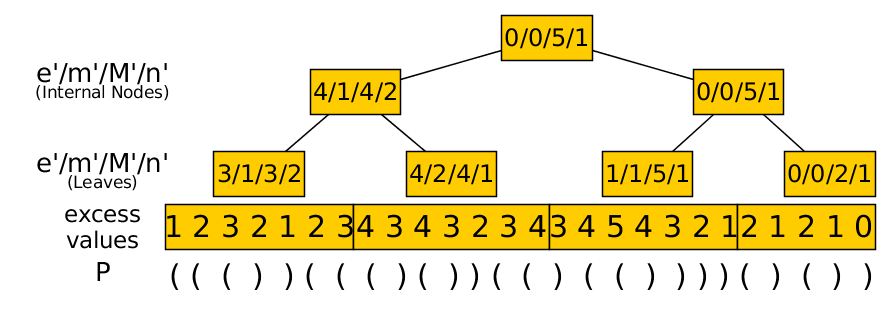
\includegraphics[scale=0.18]{./images/Range-min-max-tree.png}
  \caption{Range min-max tree}
  \label{fig:RangeMinMaxTree}
\end{figure}

Combined with a standard succinct data structure technique called {\em table
  lookup}, a {\tt RMMT} can support the primitive operations for $\pi$, as well
as $\degree$, $\child$ and $\childrank$ queries.
For example, consider $\fwdsearch(P,\pi,i,d)$.
We first check the chunk containing $P[i]$ to see if the answer is inside the
same chunk.
This can be done in constant time by constructing a universal lookup table whose
content does not depend on $P$: For each possible bit vector of length $s$,
and each of the $s$ position in the bit vector, we store the answer of
$\fwdsearch(P,\pi,i,d)$ if it can be found inside this bit vector, or $-1$
otherwise.
As there are $2^s$ bit vectors of length $s$, this table uses
$2^s\poly(s)$ bits.
If we find the  answer by performing a table lookup for the chunk containing
$P[i]$, then we return.
Otherwise, we search among the $m$ and $M$ values of the right siblings of the
leaf node $u$ corresponding to this chunk, to find the closest right sibling
that contains the answer if the answer is within chunks represented by these
siblings.
If the $m$ and $M$ values of the $k$ children of each internal node can be
packed into $O(w)$ bits, i.e., $k \lg n = O(w)$, then we can again construct
universal lookup tables for internal nodes to perform this step in constant
time.
We repeat this process until we find a right sibling, $v$, of an ancestor of $u$
whose corresponding substring of $P$ contains the answer.
We then use a similar idea to descend down the tree starting from $v$ to look
for the leaf descendant of $v$ containing the result.
Thus, we can support $\fwdsearch$ in $O(h)$ time, where $h$ is the height of the
{\tt RMMT}, provided that $k \lg n = O(w)$.

To support the primitive operations for functions $\phi$ and~$\psi$, we can
define six arrays $e'_{\phi}$, $m'_{\phi}$, $M'_{\phi}$, $e'_{\psi}$,
$m'_{\psi}$ and $M'_{\psi}$ which are similar to $e'$, $m'$ and $M'$ defined for
$\pi$ ($n'$ is defined to support $\degree$, $\child$ and $\childrank$ only, so
we need not define similar arrays for $\phi$ and $\psi$).
We make use of the following three observations to avoid storing these six
arrays explicitly: $\sumop(P, \phi, 0, i)$ and $\sumop(P, \psi, 0, i)$ are
nondecreasing, $\sumop(P, \phi, 0, i) + \sumop(P, \psi, 0, i) = i$ and
$\sumop(P, \phi, 0, i) - \sumop(P, \psi, 0, i) = \sumop(P, \pi, 0, i)$.
Thus, the each value in these six arrays can be computed in constant time
without storing them explicitly.
We only need to store the universal tables needed to support primitive
operations for $\phi$ and $\psi$.

To support $\leafrank$, $\leafselect$, $\lmostleaf$ and\break $\rmostleaf$, we
define a conceptual bit vector $P_1[1..2n]$ in which $P_1[i] = 1$ iff $P[i] = 1$
and $P[i+1] = 0$.
Hence each $1$-bit in $P_1$ corresponds to a leaf node.
The above operations then reduce to $\rankop$ and $\selop$ operations on
$P_1$, where $\rankop(P_1, i)$ returns the number of $1$s in $P_1[1..i]$ and
$\selop(P_1, i)$ returns the position of the $i$th $1$-bit in $P_1$.
For example, we have $\leafrank = \rankop(P_1, i)$.
$\rankop$ and $\selop$ operations can be further reduced to $\sumop$ and
$\fwdsearch$ for the function $\phi$ on $P_1$, which can be supported using
another range min-max tree.
Since any $O(w)$ bits in the sequence $P_1$ can be computed from $P$ in constant
time using table lookup, $P_1$ itself need not be stored explicitly, while the
cost of storing the information for the internal nodes of this range min-max
tree is dominated by the space usage of the range min-max tree for $P$.

To analyze the space usage of the entire data structure, we observe that if we
store $P$, $e'$, $m'$, $M'$ and $n'$ explicitly in a straightforward manner, the
space usage  would be $2n + \frac{k}{k-1} \cdot \frac{n}{s} \cdot \lg n$.
Navarro and Sadakane commented that choosing $s = w/2$ and $k = w / \lg n$ gives
a simple structure supporting all the operations in Table~\ref{tbl:operations}
in $O(\lg n)$ time.
However, if the trees are large enough that $w = \Theta(\lg n)$, then $e'$,
$m'$, $M'$ and $n'$ would occupy $O(n)$ bits, and the size of the representation
would be greater than is typical for a succinct tree representation,
which would use $2n+o(n)$ bits.
To reduce the overall space cost to $2n+o(n)$ bits, we can set
$s = \lceil w\lg n\rceil$ and $k = 2$.
With these parameters, looking for a potential answer to a query within a chunk
requires $O(\lg n)$ table lookups, which is dominated by the $O(\lg n)$ cost of
traversing the tree to answer queries.
Thus, the overall query cost remains $O(\lg n)$.
Moreover, for $k = 2$, universal tables are not needed for internal nodes.
Thus, we have the following lemma:

\begin{lemma}\label{lem:lg}
  An ordinal tree and its balanced parentheses sequence can be represented using
  range min-max trees in $2n + o(n)$ bits, where $n$ is the number of nodes in
  the tree.
  This structure supports all operations in Table~\ref{tbl:operations} in
  $O(\lg n)$ time.
\end{lemma}

Navarro and Sadakane showed how to use the structure described so far as a
building block for a more complicated structure that supports all operations in
Table~\ref{tbl:operations} in constant time.
Due to its complexity, however, this structure is much more difficult to
implement and may not be efficient in practice.
On the other hand, the structure described here has been experimentally verified
to be very small and achieve very good query performance in
practice~\cite{ACNSalenex10}.
This is the reason we chose this structure as the basis for our work presented
in this paper.

\subsection{Dynamic Multithreading Model}
\label{subsec:dym}
{\em Dynamic multithreading} (DYM) \cite[Chapter~27]{Cormen2009} is a
model of parallel computation that is faithful to several industry standards
such as Intel's CilkPlus (\url{cilkplus.org}), OpenMP Tasks
(\url{openmp.org/wp}), and Threading Building
Blocks (\url{threadingbuildingblocks.org}).

In this model, a {\em multithreaded computation} is modelled as a directed
acyclic graph (DAG) $G=(V,E)$ where the set of vertices $V$ are instructions
and $(u,v) \in E$ if $u$ must be executed before $v$.\footnote{Notice that the
  RAM model is a subset of the DYM model where the outdegree of every
  vertex $v \in V$ is $\leq 1$.\Norbert{Why ``$\le$''?  Doesn't the strictly
    sequential nature of the RAM model mean that everybody except the first and
    last vertices has exactly one in-neighbour and one out-neighbour?}}
The time $T_p$ needed to execute the computation on $p$ processors depends on
two parameters of the computation: its {\em work} $T_1$ and its {\em span}
$T_\infty$.
Assuming each instruction takes constant time, the work is simpy the number of
nodes (i.e., instructions) in $G$.
Since each instruction takes constant time, it clearly takes $\Theta(T_1)$ time
to execute $G$ on a single processor.
More generally, $p$ processors can execute only $p$ instructions at a time, so
$T_p = \Omega(T_1/p)$.
The span is the length of the longest path in $G$.
Since the instructions on this path need to be executed one after another, no
matter how many processors we have at our disposal, we also have
$T_p = \Omega(T_\infty)$.
Together, these two lower bounds give $T_p = \Omega(T_\infty + T_1/p)$ and
work-stealing schedulers match this lower bound to within a constant factor
(to within a factor 2 from the optimal
performance)~\cite{Blumofe:1999:SMC:324133.324234}.
The degree to which an algorithm can take advantage of the presence of $p > 1$
processors is captured by its {\em speed-up} $T_1 / T_p$ and its
{\em parallelism} $T_1 / T_\infty$.
In the absence of cache effects, the best speed-up one can hope for is $p$,
also known as {\em linear speed-up}.
The parallelism provides an upper bound on the achievable speed-up independent
of the number of available processors.

In order to describe parallel algorithms in the DYM model, we augment sequential
pseudocode with three special keywords.
The {\bf spawn} keyword, followed by a procedure call, indicates that the
procedure should run in its own thread and {\em may} thus be executed in
parallel to the thread that spawned the procedure call.
The {\bf sync} keyword indicates that the current thread must wait for the
termination of all the threads it has spawned before proceeding.
It thus provides a simple barrier-style synchronization mechanism.
Finally, {\bf parfor} is ``syntactic sugar'' for {\bf spawn}ing one thread per
iteration in a for loop, thereby allowing these iterations to run in parallel,
followed by a {\bf sync} operation that waits for all iterations to complete.
In practice, the overhead is logarithmic in the number of iterations.
If a procedure exits, either implicitly or explicitly using a {\bf return}
statement, it implicitly performs a {\bf sync} to ensure all threads it spawned
finish first.
\Norbert{Got rid of the ``strand'' stuff.
  It seems a technicality relevant only to the operation of work-stealing
  schedulers.
  If we actually use it in the analysis of the algorithm in Section 3, we
  may have to bring it back.}

%\subsection{Multicore succinct data structures}
%\label{subsec:multicoreSDS}
%A weak point of succinct data structures is their construction time,
which is generally quite slow compared to the construction time of
traditional ``pointer-linked'' data structures. We have been working
on improving construction time for succinct data structures
\cite{Fuentes2014}. In that paper, two practical multicore algorithms
for wavelet tree construction were introduced. Both algorithms run
have $O(n\lg \sigma)$ {\em work} time and $O(n)$ {\em span}, where $n$
is the input size and $\sigma$ is the alphabet size. In
\cite{DBLP:journals/corr/Shun14}, Shun introduced 3 new algorithms to
construct wavelet trees in parallel. The best algorithm, in practice,
has $O(n\lg \sigma)$ {\em work} time and $O(\lg n\lg \sigma)$ {\em
span}. Shun also explain how to parallelize the construction of
rank/select structures, taking $O(n)$ {\em work} time and $O(1)$ {\em
span} for rank structures and $O(n)$ {\em work} time and $O(\lg n)$
{\em span} for select structures. The author does not provide an
implementation of its proposal.

%%%%%%%%%%%%%%%%%%%%%%%%%%%%%%%%%%%
%%%%% MULTICORE SUCCINCT TREE %%%%%
%%%%%%%%%%%%%%%%%%%%%%%%%%%%%%%%%%%

\section{Multicore Succinct Tree}
\label{sec:multicoreST}
% We will focus on polylogarithmic-size trees because they are the
% only ones that have an implementation we can compare ourselves to;
% in particular, we take the {\tt
% libcds}\footnote{\url{http://libcds.recoded.cl}. We thank Diego
% Arroyuelo for the conversations about the implementation of succinct
% trees.}\cite{ACNSalenex10} and {\tt
% sdsl}\footnote{\url{https://github.com/simongog/sdsl-lite}}
% libraries as state-of-the-art and our sequential baseline.
%
% \Jose{In this section I'll use the same notation used in
% \cite{Navarro:2014:FFS:2620785.2601073}. This notation should be
% introduced in the Related Work section}\\


\subsection{Parallel Succinct Tree}
\label{sec:PST}

\subsubsection{The idea}
\label{subsec:idea}
We propose a parallel algorithm based in the construction of the
\emph{Range Min-Max Tree}, {\tt
  RMMT}. Our algorithm, called
\emph{Parallel Succinct Tree Algorithm}, {\tt PSTA}, has as input a
tree on $n$ nodes stored as a sequence of balanced parentheses, $P$, of
size $2n$.

%The {\tt RMMT} is constructed over $P$, partitioning $P$ in disjoint
%chunks of size $s$. Considering those chunks, the construction of the
%{\tt RMMT} is based in the computation of different arrays of size
%$O(\frac{N}{s})$. Such arrays are $e^{\prime}$, saving the final
%excess of each chunk, $m^{\prime}$, saving the minimum excess value of
%each chunk, $M^{\prime}$, saving the maximum excess value of each
%chunk and $n^{\prime}$, saving the number of ocurrences of the minimum
%value of each chunk. As a reminder, the excess value at position $i$
%is:
%\begin{equation}
%  \displaystyle E[i] = \sum_{k=0}^{i} \pi(P[k])
%  \label{eq:excess}
%\end{equation}

%where $\pi(``(") = 1$ and $\pi(``)") = -1$. See Figure
%\ref{fig:RangeMinMaxTree} as an example of {\tt RMMT}, with $s=3$ and
%$k=3$.

%\begin{figure}[ht]
%  \centering
%  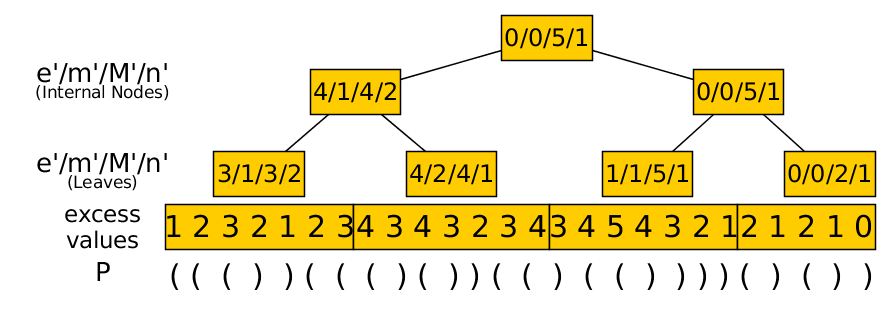
\includegraphics[scale=0.18]{./images/Range-min-max-tree.png}
%  \caption{Range min-max tree}
%  \label{fig:RangeMinMaxTree} 
%\end{figure}

The first step of {\tt PSTA} is to compute the arrays $e^{\prime}$,
$m^{\prime}$, $M^{\prime}$ and $n^{\prime}$ in parallel. Since
$e^{\prime}$ just saves the last excess value of each chunk, which is
a sum, {\tt PSTA} needs to apply a parallel prefix sum
algorithm. Computing the last element of $e^{\prime}$, at position
$\frac{2n}{s}-1$, we indirectly compute the rest of the elements of
$e^{\prime}$. We adapted the algorithm in \cite{Helman2001265} for
this context, computing $e^{\prime}$ in $O(\frac{n}{p}+\lg p)$ time, using
$p$ threads. Note that we do not need to compute more elements of
$e^{\prime}$ to the internal nodes of the {\tt RMMT}. The memory used
in construction time are bounded by $O(n\lg(n))$ bits.

To compute $m^{\prime}$, let's assume, without loss of generality,
that $p = k^{i}$, where $k$ is the arity
of the internal nodes in the {\tt RMMT} and $i > 0$. {\tt PSTA}
assigns one thread per sub-tree of size $O(\frac{n}{sp})$, at level
$i$. So, it is possible to compute the $m^{\prime}$ values in all
sub-trees, in parallel, in $O(\frac{n}{sp}k)$ time. Then, for the
rest $O(p)$ nodes in the top of the tree, we compute the corresponding
minimum values in $O(k\lg_{k} p)$ time, computing each level in $O(k)$
time, just looking the $k$ values on the previous level using one
thread per vertex. If we consider $s$ and $k$ as constants, we can compute
$m^{\prime}$ in
$O(\frac{n}{sp}k + \lg p) = O(\frac{n}{p}+\lg p)$ \Jose{$s$ and $k$ constants?}time,
using $O(n\lg(n))$ bits in construction time and in the
final array. Note that this solution makes sense considering that
$p\ll N$. Figure \ref{fig:min-max-array} illustrates the solution
explained here. We can compute $M^{\prime}$ and $n^{\prime}$ in the
same way, obtaining the same complexity.

\begin{figure}[t]
  \centering
  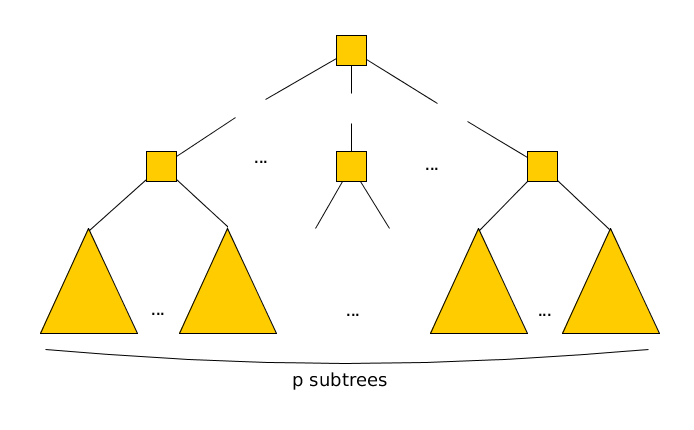
\includegraphics[scale=0.28]{./images/Min-Max-array.png}
  \caption{Computation of $m^{\prime}$ and $M^{\prime}$}
  \label{fig:min-max-array} 
\end{figure}

In addition to the arrays, the construction of the {\tt RMMT} involves
the computation of \emph{universal tables}.
%The universal tables are
%used to support \emph{fwd\_search}($\bullet$),
%\emph{bwd\_search}($\bullet$), \emph{rmqi}($\bullet$),
%\emph{RMQi}($\bullet$), \emph{degree}($\bullet$) and
%\emph{child}($\bullet$) queries.
We can divide
universal tables into two types: those that depend on the leaves of
the {\tt RMMT} and those that depend on the internal nodes. In the
first case, we can compute each universal table in parallel assigning
one processor per leaf or chunk, which allows to compute different
parts of the table at the same time. For the second kind of tables, we
can assign one processor per internal node. Such processor computes
the section corresponding to that internal node in the universal
table. In that way, since computing the universal tables sequentially
has a complexity of $O(\sqrt{2^{w}}poly(w))$ time according to
\cite{Navarro:2014:FFS:2620785.2601073}, we can compute those
universal tables in $\displaystyle O(\frac{\sqrt{2^{w}}poly(w)}{p})$,
using $p$ processors.

To reduce the space used by the {\tt RMMT}, Sadakane and Nava\-rro used
the \emph{aB-tree}. As the {\tt RMMT} and aB-tree are both complete trees, we can apply a
construction as that shown in Figure \ref{fig:min-max-array} to
construct the aB-tree. With respect to the universal tables needed in
the aB-tree, they can be computed following the same strategy
explained previously, but now with size $O(\sqrt{2^{w}})$
bits.

Finally, we can modify Theorem 4 of
\cite{Navarro:2014:FFS:2620785.2601073} as follows:

\newtheorem{theorem}{Theorem}
\begin{theorem}
  We can represent a parentheses sequence $P$ of size $2n$, computing all
  operations of Table \ref{tbl:operations}
  in $O(\lg n)$ time, with a data
  structure depending on $P$ that uses $2n+o(n)$ bits, and universal
  tables (i.e., not depending on $P$) that use $O(\sqrt{2^{w}}poly(w))$
  bits, where $w$ is the word size of the RAM model. The preprocessing
  time is $O(\frac{n}{p} + \lg p)$, using $p$
  processors, and its working space is $O(n\lg n)$ bits.
\end{theorem}
			
When we talk about a $w$-bit word RAM, we mean a model that supports
parallelism and can manipulate $w$ bits in $O(1)$. DYM meets these
criteria. Additionally, we consider that the overhead (in space and
time) imposed by the scheduling of processors is negligible. This is
reflected in the results of \cite{Blumofe:1999:SMC:324133.324234} and in the fact that the number of available processing units in current systems is generally much lower than the input $n$.


\subsubsection{Parallel Succinct Tree Algorithm}
\label{subsec:multicoreSTAlgorithm}
The {\tt PSTA} algorithm is shown in Algorithm \ref{algo:PSTA1},
\ref{algo:PSTA2} and \ref{algo:PSTA3}. Algorithm \ref{algo:PSTA1}
shows the computation of the leaves of the {\tt RMMT}, Algorithm
\ref{algo:PSTA2} shows the computation of the internal nodes of the
{\tt RMMT} and finally Algorithm \ref{algo:PSTA3} shows the
computation of the universal tables. The sequential version of {\tt
  PSTA} can be obtained by replacing {\bf parfor} instruction with
sequential {\bf for} instructions. The algorithm takes as input a parentheses
sequence $P$ of size $2n$, the arity $k$ of the internal nodes in the {\tt
  RMMT}, the size of each chunk $s$ and the total numbers of available
threads. In the sequence $P$, opened-parenthesis and
closed-parenthesis are coded by a $1$ and a $0$, respectively. The
output is the {\tt RMMT} represented by its arrays $e^{\prime}$,
$m^{\prime}$, $M^{\prime}$, $n^{\prime}$ and universal tables to
support queries in $O(\lg n)$ time.

Let's first analyze Algorithm \ref{algo:PSTA1}. Since the {\tt RMMT}
can be seen as a complete tree of arity $k$, it is easy to calculate
the size of the arrays $e^{\prime}$, $m^{\prime}$, $M^{\prime}$ and
$n^{\prime}$. The size of array $e^{\prime}$ is the number of leaves
in the {\tt RMMT} (line 2). The size of arrays $m^{\prime}$,
$M^{\prime}$ and $n^{\prime}$ is equal to the total number of nodes in
the {\tt RMMT}; that is, $\frac{\lceil 2n/s \rceil-1}{k-1} + \lceil
2n/s \rceil$ (lines 1 and 3). Lines 4 to 26 shows the computation of
partial excess values in parallel. The first step is to compute the
number of chunks that each thread has to process (line 4). Then, in
parallel, each thread computes the excess value of $ct$ consecutive
chunks, following the equation to compute excess values. In each chunk, the
thread increases by one its partial excess value each time that an
open parenthesis appears, and decreases by one in the other case
(lines 12 to 15). Immediately after the partial excess changes, it is
necessary to verify if the maximum, minimum and number of minimum
values also change (lines 16 to 22). When a chunk is completed, the
local excess and its associated values are stored in the arrays
$e^{\prime}$, $m^{\prime}$, $M^{\prime}$ and $n^{\prime}$ (lines 23 to
26). After a thread finishes processing its chunks, it is necessary to
complement its local excess values considering the local values of
previous threads. To do that, we first update the final excess value
of each thread using a parallel prefix sum algorithm (line 27). 
Those excess values do not need to be modified again. Observe that
the prefix sum algorithm only needs to consider $p$ values, at positions
$i*ct-1$, with $1\leq i \leq p-1$. Due to the updated final excess value,
each thread can update the other excess, minimum and maximum values in
parallel (lines 28 to 33). At this point, {\tt PSTA} has computed all
the leaves of the {\tt RMMT} in parallel.

Algorithm \ref{algo:PSTA2} shows the computation of the internal
nodes, which has two substeps: The first substep computes $O(p)$
subtrees in parallel (lines 2 to 18) and the second one computes the
top of the {\tt RMMT} (lines 19 to 34). To ensure that $O(p)$ subtrees
will be computed in parallel, it is necessary to compute the closest
level to the root that has at least $p$ subtrees (line 1). After that,
{\tt PSTA} computes in parallel each subtree at that level. Each
thread computes each node of the corresponding subtree by scanning the
$k$ children of that node, obtaining the corresponding minimum and
maximum values (lines 3 to 18). Notice that one thread can compute
more than one subtree and those subtrees can be non-consecutive. With
a scheduler that balances the work, such as a work-stealing scheduler,
threads have a similar workload. In the second substep, the $O(\lceil
\log_{k}p \rceil)$ levels of the top of the {\tt RMMT} are computed in
parallel. The {\tt PSTA} algorithm assigns one node per thread,
computing each level in $O(k)$ time.

In the last step of {\tt PSTA}, Algorithm \ref{algo:PSTA3} shows the computation of
universal tables. To simplify the explanation, Algorithm
\ref{algo:PSTA3} just shows the computation of one universal table,
$near\_fwd\_pos$, used to compute the \emph{fwd\_ search} operation. The same algorithm can be applied to the other
tables. All of these tables do not depend on the input, except for the
number of available threads.
\begin{minipage}[t]{.50\textwidth}
  \vspace{0pt}  
  \begin{algorithm}[H]
\small
\SetVlineSkip{-2cm}
  % keywords
  \SetKwInOut{Input}{Input}
  \SetKwInOut{output}{output}
  \SetKwFor{PFor}{parfor}{do}{end}
  \LinesNumbered
  \SetAlgoNoEnd
  \DontPrintSemicolon
  % I/o
  \Input{$P$, $k$, $s$, $threads$}
  \output{$e^{\prime}, m^{\prime}, M^{\prime}, n^{\prime}$ and universal tables ({\tt RMMT})}
  \BlankLine% \SetAlgoNoLine
  % algorithm
  $o$ = $\frac{\lceil 2n/s \rceil-1}{k-1}$\tcp*[h]{\# internal nodes}\;
  $e^{\prime}$ = array of size $\lceil 2n/s \rceil$\;
  $m^{\prime}, M^{\prime}, n^{\prime}$ = arrays of size $\lceil 2n/s \rceil + o$\;
  $ct$ = $\lceil 2n/s \rceil/threads$\;%\tcp*[h]{Chunks per thread}\;
  \PFor{$t\leftarrow 0$ \KwTo $threads-1$}{
	  $e^{\prime}_t, m^{\prime}_t, M^{\prime}_t, n^{\prime}_t$ = $0$\;
	  
	  \For{$chk \leftarrow 0$ \KwTo $ct$}{
		  $low$ = $t*ct*s+chk*s$\;
		  $up$ = $low+s$\;
	  	
		  \For{$par \leftarrow low$ \KwTo $up$}{
		  	\eIf{$P[par]$ is $closed$}{
		  		$e^{\prime}_t$ -= $1$\;
		  	}
		    {
		  		$e^{\prime}_t$ += $1$\;
		    }
		    
		    \uIf{$e^{\prime}_t < m^{\prime}_t$}{
				$m^{\prime}_t$ = $e^{\prime}_t$\;
				$n^{\prime}_t$ = $1$
			}
			\uElseIf{$e^{\prime}_t == m^{\prime}_t$}{
				$n^{\prime}_t$ += $1$\;
			}
			\uElseIf{$e^{\prime}_t > M^{\prime}_t$}{
				$M^{\prime}_t$ = $e^{\prime}_t$\;
			}
		  }
		  $e^{\prime}[t*ct+chk]$ = $e^{\prime}_t$\;
		  $m^{\prime}[t*ct+chk+o]$ = $m^{\prime}_t$\;
		  $M^{\prime}[t*ct+chk+o]$ = $M^{\prime}_t$\;
		  $n^{\prime}[t*ct+chk+o]$ = $n^{\prime}_t$\;		  
	  }
  }
  \BlankLine
  $parallel\_prefix\_sum(e^{\prime}, ct)$\;
%  \For{$t \leftarrow 1$ \KwTo $threads-1$}{
%		$e^{\prime}[(t+1)*ct-1]$ += $e^{\prime}[t*ct-1]$\;
 % }
  \BlankLine
  \PFor{$t\leftarrow 1$ \KwTo $threads-1$}{
	  \For{$chk \leftarrow 0$ \KwTo $ct$}{
	  	\If{$t == threads-1$ OR $chk < ct-1$}{
	  	  $e^{\prime}[t*ct+chk]$ += $e^{\prime}[t*ct-1]$\;
	  	}
  	  	$m^{\prime}[t*ct+chk+o]$ += $e^{\prime}[t*ct-1]$\;
  	  	$M^{\prime}[t*ct+chk+o]$ += $e^{\prime}[t*ct-1]$\;
	  }
  }
%  \Return{$WT$}\;
  \caption{{\tt PSTA} (part I)}
  \label{algo:PSTA1}
  \end{algorithm}
\end{minipage}%
%hfill
\begin{minipage}[t]{.51\textwidth}
  \vspace{0pt}
  \begin{algorithm}[H]
\small
\SetVlineSkip{-2cm}
  % keywords
%  \SetKwInOut{Input}{Input}
%  \SetKwInOut{output}{output}
  \SetKwFor{PFor}{parfor}{do}{end}
  \LinesNumbered
  \SetAlgoNoEnd
  \DontPrintSemicolon
  % I/o
%  \Input{Parentheses sequence $P$, $k$, $s$, $threads$}
%  \output{$e^{\prime}, m^{\prime}, M^{\prime}, n^{\prime}$ and universal tables ({\tt RMMT})}
%  \BlankLine%
  \SetAlgoLined
%\setcounter{AlgoLine}{2}
%\ShowLn
  % algorithm
  \setcounter{AlgoLine}{1}\ShowLn
  $lvl$ = $\lceil \log_{k}threads \rceil$\;
  \setcounter{AlgoLine}{2}\ShowLn
  \PFor{$st\leftarrow 0$ \KwTo $k^{lvl}$}{
      \setcounter{AlgoLine}{3}\ShowLn
	  \For{$l\leftarrow \lceil\log_{k}(2n/s)\rceil-1$ \KwTo $lvl$}{
          \setcounter{AlgoLine}{5}\ShowLn
		  \For{$d\leftarrow 0$ \KwTo $k^{l-lvl}$}{
            \setcounter{AlgoLine}{5}\ShowLn
		  	$i$ = $d + k^{l} - 1 +st*k^{l-lvl}$\;
            \setcounter{AlgoLine}{6}\ShowLn
		  	$b$ = $i*k+1$\;
            \setcounter{AlgoLine}{7}\ShowLn
			\For{$c\leftarrow b$ \KwTo $b+k-1$}{
%****
                \setcounter{AlgoLine}{8}\ShowLn
			  	\uIf{$c == b$}{
                  \setcounter{AlgoLine}{9}\ShowLn
				  $m^{\prime}[i]$ = $m^{\prime}[c]$\;
                  \setcounter{AlgoLine}{10}\ShowLn
				  $M^{\prime}[i]$ = $M^{\prime}[c]$\;
                  \setcounter{AlgoLine}{11}\ShowLn
				  $n^{\prime}[i]$ = $n^{\prime}[c]$\;					
			  	}
                \setcounter{AlgoLine}{12}\ShowLn
			    \uElseIf{$m^{\prime}[c] < m^{\prime}[i]$}{
                    \setcounter{AlgoLine}{13}\ShowLn
					$m^{\prime}[i]$ = $m^{\prime}[c]$\;
                    \setcounter{AlgoLine}{14}\ShowLn
					$n^{\prime}[i]$ = $n^{\prime}[c]$\;
				}
                \setcounter{AlgoLine}{15}\ShowLn
				\uElseIf{$m^{\prime}[c] == m^{\prime}[i]$}{
                    \setcounter{AlgoLine}{16}\ShowLn
					$n^{\prime}[i]$ += $n^{\prime}[c]$\;
				}
                \setcounter{AlgoLine}{17}\ShowLn
				\uElseIf{$M^{\prime}[c] > M^{\prime}[i]$}{
                    \setcounter{AlgoLine}{18}\ShowLn
					$M^{\prime}[i]$ = $M^{\prime}[c]$\;
				}
%****
		    						
%			  	\eIf{$c == b$}{
%				  $m^{\prime}[i]$ = $m^{\prime}[c]$\;
%				  $M^{\prime}[i]$ = $M^{\prime}[c]$\;
%				  $n^{\prime}[i]$ = $n^{\prime}[c]$\;					
%			  	}
%			    	{
%				    \uIf{$m^{\prime}[c] < m^{\prime}[i]$}{
%						$m^{\prime}[i]$ = $m^{\prime}[c]$\;
%						$n^{\prime}[i]$ = $n^{\prime}[c]$\;
%					}
%					\uElseIf{$m^{\prime}[c] == m^{\prime}[i]$}{
%						$n^{\prime}[i]$ += $n^{\prime}[c]$\;
%					}
%					\uElseIf{$M^{\prime}[c] > M^{\prime}[i]$}{
%						$M^{\prime}[i]$ = $M^{\prime}[c]$\;
%					}
%		    		}
			}		  	
		  }
	  }
  }
  \BlankLine
  \setcounter{AlgoLine}{19}\ShowLn
  \For{$l\leftarrow lvl-1$ \KwTo $0$}{
	  \setcounter{AlgoLine}{20}\ShowLn
	  \PFor{$d\leftarrow 0$ \KwTo $k^{l}$}{
        \setcounter{AlgoLine}{21}\ShowLn
	  	$i$ = $d + (k^{l}-1)/(k-1)$\;
        \setcounter{AlgoLine}{22}\ShowLn
	  	$b$ = $i*k+1$\;
        \setcounter{AlgoLine}{23}\ShowLn
		\For{$c\leftarrow b$ \KwTo $b+k-1$}{
%****		
            \setcounter{AlgoLine}{24}\ShowLn
		  	\uIf{$ch == b$}{
              \setcounter{AlgoLine}{25}\ShowLn
			  $m^{\prime}[i]$ = $m^{\prime}[c]$\;
              \setcounter{AlgoLine}{26}\ShowLn
			  $M^{\prime}[i]$ = $M^{\prime}[c]$\;
              \setcounter{AlgoLine}{27}\ShowLn
			  $n^{\prime}[i]$ = $n^{\prime}[c]$\;					
		  	}
            \setcounter{AlgoLine}{28}\ShowLn
		    \uElseIf{$m^{\prime}[c] < m^{\prime}[i]$}{
                \setcounter{AlgoLine}{29}\ShowLn
				$m^{\prime}[i]$ = $m^{\prime}[c]$\;
                \setcounter{AlgoLine}{30}\ShowLn
				$n^{\prime}[i]$ = $n^{\prime}[c]$\;
			}
            \setcounter{AlgoLine}{31}\ShowLn
			\uElseIf{$m^{\prime}[c] == m^{\prime}[i]$}{
                \setcounter{AlgoLine}{32}\ShowLn
				$n^{\prime}[i]$ += $n^{\prime}[c]$\;
			}
            \setcounter{AlgoLine}{33}\ShowLn
			\uElseIf{$M^{\prime}[c] > M^{\prime}[i]$}{
                \setcounter{AlgoLine}{34}\ShowLn
				$M^{\prime}[i]$ = $M^{\prime}[c]$\;
			}
%****		
	    		
%		  	\eIf{$ch == b$}{
%			  $m^{\prime}[i]$ = $m^{\prime}[c]$\;
%			  $M^{\prime}[i]$ = $M^{\prime}[c]$\;
%			  $n^{\prime}[i]$ = $n^{\prime}[c]$\;					
%		  	}
%		    	{
%			    \uIf{$m^{\prime}[c] < m^{\prime}[i]$}{
%					$m^{\prime}[i]$ = $m^{\prime}[c]$\;
%					$n^{\prime}[i]$ = $n^{\prime}[c]$\;
%				}
%				\uElseIf{$m^{\prime}[c] == m^{\prime}[i]$}{
%					$n^{\prime}[i]$ += $n^{\prime}[c]$\;
%				}
%				\uElseIf{$M^{\prime}[c] > M^{\prime}[i]$}{
%					$M^{\prime}[i]$ = $M^{\prime}[c]$\;
%				}
%	    		}
		}		  	
	  }
  }
  \caption{{\tt PSTA} (part II)}
  \label{algo:PSTA2}
	  \end{algorithm}
\end{minipage}

\subsubsection{Theoretical Analysis}
\label{subsec:theoreticalAnalysis}
The sequential version of {\tt PSTA} takes $O(N+\sqrt{2^{w}}poly(w))$,
the same complexity reported in
\cite{Navarro:2014:FFS:2620785.2601073}. The amount of work of {\tt
PSTA}, $T_1$, is the aggregation of the amount of work of Algorithms \ref{algo:PSTA1},
\ref{algo:PSTA2} and \ref{algo:PSTA2}. The work of Algorithm \ref{algo:PSTA1} is $O(N)$,
since that it behaves as a sequential list ranking algorithm (all the computation is
done in lines 8 to 26). The work of Algorithm \ref{algo:PSTA2} is $O(\frac{N}{s})$. Here,
all the computation is done in the first part (lines 1 to 18), having only one
subtree which contains all internal nodes of the {\tt RMMT}. The work of Algorithm \ref{algo:PSTA3} is equivalent to compute all universal tables sequentially, mantaining
the complexity in \cite{Navarro:2014:FFS:2620785.2601073}, that is, $O(\sqrt{2^{w}}poly(w))$. Therefore, the amount of work of {\tt PSTA} is $T_{1}=O(N+\sqrt{2^{w}}poly(w))$. Considering $p$ processors, the first part of Algorithm \ref{algo:PSTA1} (lines 5 to 26) as a complexity of $O(\frac{N}{p})$. Meanwhile, the second part (line 27) has a complexity of $O(\lg p)$ if we use the parallel list ranking algorithm in \cite{Reif1993}. Finally, the third part of Algorithm \ref{algo:PSTA1} (lines 28 to 33) has a complexity of $O(\frac{N}{sp})$. On the other hand, the first half of Algorithm \ref{algo:PSTA2} (lines 1 to 18) has a complexity of $O(\frac{Nk}{sp})$ and the second half (lines 19 to 34) has a complexity of $O(k\lg_{k}p)$. Algorithm \ref{algo:PSTA3} has a complexity of $O(\frac{\sqrt{2^{w}}poly(w)}{p})$. Therefore, the complexity of {\tt PSTA} with $p$ available processors is $T_p =
O(\frac{N}{p}+\lg p+\frac{\sqrt{2^{w}}poly(w)}{p})$, considering $s$ and $k$ constants. Now, if we consider that we have enough amount of processors, the span of {\tt PSTA} is $T_{\infty}=O(\lg N)$. Here, the span of the whole algorithm is the maximum span of all its parts. The span of Algorithm \ref{algo:PSTA1} is $O(\lg N)$, since all the computation is done in the parallel list ranking algorithm (line 27). In Algorithm \ref{algo:PSTA2} all the computation is centered in the second half, with span $O(k\lg_{k}N)$. In Algorithm \ref{algo:PSTA3}, since each cell of the universal tables can be computed independently of the rest, the span if $O(1)$. Note that the overhead implicit in each {\bf parfor} does not affect the previous complexities.

Since we have the three metrics provided by the DYM model, we can
compute speedup and parallelism. The speedup of our algorithm is $T_1/T_P$ =
$O(\frac{p(N+\sqrt{2^{w}}poly(w))}{N+\sqrt{2^{w}}poly(w)+p\lg p})$. As we can see,
under the assumption of $p\ll N$, the speedup tends to $O(p)$. The assumption
$p\ll N$ is realistic, especially considering current SMP-like
systems, where the amount of available processing units is much less than the
input, $N$ in this case. The parallelism of {\tt PSTA} is $T_1/T_{\infty}$ =
$\frac{N+\sqrt{2^{w}}poly(w)}{\lg N}$ \Jose{...}

An important advantage of our algorithm is its working space. The {\tt
PSTA} algorithm does not need any extra memory related to the usage of
threads. Indeed, it just needs a working space proportional to the
input size and the space needed to schedule the threads. A
work-stealing scheduler, as that used by the DYM model, exhibit at
most a linear expansion space, that is, $O(S_1p)$, where $S_1$ is the
minimum amount of space used by the scheduler for any execution of a
multithreaded computation using one processor. This upper bound is
optimal to within a constant factor
\cite{Blumofe:1999:SMC:324133.324234}. In summary, the working space
needed by our algorithm is $O(N+S_1p)$. Thus, considering the
assumption $p\ll N$, the working space is dominated by the input
size. The scheduling space is negligible.

The algorithm reaches its optimal behavior when the work of building
each subtree in parallel (lines 2 to 18 of Algorithm \ref{algo:PSTA2})
is the same as the work needed to create the top part of the {\tt
RMMT} (lines 19 to 32 of Algorithm \ref{algo:PSTA2}). This point is
reached when the $p\log_{k}p=N/s$. 

%\subsection{Parallel Succinct Tree for Large Trees}
%\label{subsec:parallelLargeTrees}
%\input{parallelLargeTrees}

\subsection{Parallel Folklore Encoding Algorithm}
\label{subsec:parenthesesAlgorithm}
As we mentioned above, the input to {\tt RMMT} consists of a
parentheses sequence $P$. However, sometimes $P$ is not available,
instead we have un ordinal tree, $T$. The construction of $P$ from $T$
has not been considered in previous implementations of the {\tt
  RMMT}. Here, we proposed an algorithm to compute $P$ in parallel,
complementing the {\tt PSTA} algorithm. We will call this algorithm
\emph{Parallel Folklore Enconding Algorithm}, {\tt PFEA}. The key
observation to obtain $P$ is that each parenthesis associated to an
edge $(u,v)$, ``('' or ``)'', is followed in the enconding by a
parenthesis associated to the edge $(parent(u), v)$, $(v, first(v))$
or $(u, next(u,v))$. All of them at distance of 1 of the edge
$(u,v)$. In the observation, $parent(u)$ is the parent node $u$,
$first(v)$ is the first child of $v$ and $next(u,v)$ is the child of
$u$ that succeeds the node $v$ in the array or children. With this
observation in mind, the core of {\tt PFEA} works as follows: Let
$(u,v)$ be an edge of $T$, where $u$ is parent of $v$ and let
$(u,v)_{0}$ ($(u,v)_{1}$) the opened (closed) parenthesis associated
to $(u,v)$. First, if $v$ is a leaf, then $(u,v)_{0}$ is followed by
$(u,v)_{1}$. If $v$ is not a leaf, then $(u,v)_{0}$ is followed by
$(v,first(v))_{0}$. If $v$ is not the last child of $u$,then
$(u,v)_{1}$ is followed by $(u,next(u,v))_{0}$. Finally, if $v$ is the
last child of $u$, then $(u,v)_{1}$ is followed by
$(u,parent(u))_{1}$. 

\begin{algorithm}[t]
\small
\SetVlineSkip{-2cm}
  % keywords
  \SetKwInOut{Input}{Input}
  \SetKwInOut{output}{output}
  \SetKwFor{PFor}{parfor}{do}{end}
  \LinesNumbered
  \SetAlgoNoEnd
  \DontPrintSemicolon
  % I/o
  \Input{Arrays $V$ and $E$ representing the ordinal tree $T$}
  \output{Parentheses sequence representation of $T$}
  \BlankLine% \SetAlgoNoLine
  % algorithm
  $ET, P$ = arrays of size $2|E|$\;
  \PFor{$i\leftarrow 0$ \KwTo $|E|-1$}{
  	$orig = E[i].origin$,
  	$dest = E[i].destiny$\;
  	$ET[2i].value = 0$\tcp*[h]{(}\;
  	$ET[2i+1].value = 1$\tcp*[h]{)}\;
  	
  	\eIf{$dest.node$ is a $leaf$}{
  		$ET[2i].succ = ET[2i+1]$\;
	}
	{
  		$ET[2i].succ = ET[2*next(dest.node,dest.index)]$\;
    }
  \BlankLine
  	\eIf{$orig$ is a last incident egde}{
  		$ET[2i+1].succ = ET[2*parent(orig.node)+1]$\;
	}
	{
  		$ET[2i+1].succ = ET[2*next(orig.node,orig.index)]$\;
    }
  }
  \BlankLine
  $parallel\_list\_ranking(ET)$\;
  \BlankLine
  \PFor{$i\leftarrow 0$ \KwTo $2|E|-1$}{
  	$P[ET[i].rank] = ET[i].value$
  }
  \caption{{\tt PFEA}}
  \label{algo:PFEA}
\end{algorithm}
\normalsize


%%%%%%%%%%%%%%%%%%%%%%%
%%%%% EXPERIMENTS %%%%%
%%%%%%%%%%%%%%%%%%%%%%%

\section{Experimental Results}
\label{sec:exps}
To evaluate the performance of our {\tt PSTA} algorithm, we compare it against
{\tt libcds}~\cite{libcds} and {\tt sdsl}~\cite{sdsl}, which are
state-of-the-art implementations of the {\tt RMMT}.
Both assume that the input tree is given as a parenthesis sequence, as we do
here.
Our implementation of the {\tt PSTA} algorithm deviates from the description in
Section~\ref{sec:multicoreST} in that the prefix sum computation in
line~22 of the algorithm is done sequentially in our implementation.
This changes the running time to $O(n/p + p)$ but simplifies the implementation.
Since $p \ll n/p$ for the input sizes we are interested in and the numbers of
cores available on current multicore systems, the impact on the running
time is insignificant.


\subsection{Experimental Setup}
\label{subsec:experimentalSetup}
We implemented the {\tt PSTA} algorithm in C and compiled it using GCC 4.9 with
optimization level -O2 and using the \mbox{-ffast-math flag}.\footnote{The code
  and data needed to replicate our results are available at
  \url{http://www.inf.udec.cl/~josefuentes/spaa2015}.}
All parallel code was compiled using the GCC Cilk branch.
The same flags were used to compile {\tt libcds} and {\tt sdsl}, which were
written in C++.

We tested our algorithm on five inputs.
The first two were suffix trees of the DNA ({\tt dna}, 1,154,482,174
parentheses), and protein ({\tt prot}, 670,721,006 parentheses) data from the
Pizza \& Chili corpus\footnote{\url{http://pizzachili.dcc.uchile.cl}}.
These suffix tree were constructed using code from
\url{http://www.daimi.au.dk/~mailund/suffix_tree.html}.
The next two inputs were XML trees of the Wikipedia
dump\footnote{\url{http://dumps.wikimedia.org/enwiki/20150112/enwiki-20150112-pages-articles.xml.bz2} (January 12, 2015)}
({\tt wiki}, 498,753,914 parentheses) and OpenStreetMap
dump\footnote{\url{http://wiki.openstreetmap.org/wiki/Planet.osm} (January 10,
  2015)} ({\tt osm}, 4,675,776,358 parentheses).
The final input was a complete binary tree of depth 30 ({\tt ctree},
2,147,483,644 parentheses).

The experiments were carried out on a machine with four 16-core AMD
Opteron\texttrademark{} 6278 processors clocked at 2.4GHz,
with 64KB of L1 cache per core, 2MB of L2 cache shared
between two cores, and 6MB of L3 cache shared between 8 cores.
The machine had 189GB of DDR3 RAM, clocked at 1333MHz.

The running times of the algorithms were measured using
the high-resolution (nanosecond) C functions in {\tt <time.h>}.
Memory consumption was measured using the tools provided by
{\tt malloc\_count} \cite{malloc-count}.
In our experiments, the chunk size $s$ and the arity $k$ were fixed at 256 and
2, respectively.


\subsection{Results and Discussion}
\label{subsec:resultsDiscussion}
\stepcounter{footnote}\newcounter{pizzachili}\setcounter{pizzachili}{\value{footnote}}
\stepcounter{footnote}\newcounter{xmldata}\setcounter{xmldata}{\value{footnote}}
\setlength{\tabcolsep}{3pt}
\begin{table*}[ht]
  \centering
  \begin{tabular}{crrrrrrrrrrrrrrr}
    & \multicolumn{3}{c}{xml} & \multicolumn{3}{c}{dna} & \multicolumn{3}{c}{psd7003} & \multicolumn{3}{c}{protein} & \multicolumn{3}{c}{comptree}\\
    &  \multicolumn{3}{c}{(23,551,472)} & \multicolumn{3}{c}{(32,747,474)} & \multicolumn{3}{c}{(42,611,636)} & \multicolumn{3}{c}{(60,160,372)} & \multicolumn{3}{c}{(2,147,483,646)}\\
\hline
    $p$ & \verb|psta| & \verb|libcds| & \verb|sdsl|  & \verb|psta| & \verb|libcds| & \verb|sdsl| & \verb|psta| & \verb|libcds| & \verb|sdsl| & \verb|psta| & \verb|libcds| & \verb|sdsl| & \verb|psta| & \verb|libcds| & \verb|sdsl|\\
\hline
 1   &  .99  &  9.95  & .60  &  1.01 & 10.68  & .64  &  1.04  & 10.73  & .63  &  .99   &  10.16  &  .61   & 1.00  & 11.59  & .69   \\
 2   &  1.96 &  19.71 & 1.19 &  1.98 & 21.01  & 1.27 &  2.06  & 21.33  & 1.26 &  1.98  &  20.26  &  1.22  & 1.98  & 22.93  & 1.36  \\
 4   &  3.77 &  38.00 & 2.30 &  3.88 & 41.18  & 2.48 &  3.94  & 40.84  & 2.41 &  3.92  &  39.99  &  2.41  & 3.82  & 44.33  & 2.62  \\
 6   &  5.25 &  52.84 & 3.20 &  5.43 & 57.73  & 3.48 &  5.63  & 58.30  & 3.44 &  5.46  &  55.77  &  3.36  & 5.50  & 63.82  & 3.78  \\
 8   &  7.14 &  71.89 & 4.36 &  7.30 & 77.58  & 4.67 &  6.89  & 71.36  & 4.21 &  7.49  &  76.45  &  4.60  & 7.64  & 88.64  & 5.25  \\
 10  &  8.09 &  81.46 & 4.94 &  8.42 & 89.43  & 5.39 &  6.72  & 69.66  & 4.11 &  7.14  &  72.97  &  4.39  & 9.14  & 106.01 & 6.28  \\
 12  &  7.58 &  76.38 & 4.63 &  7.83 & 83.19  & 5.01 &  7.97  & 82.59  & 4.87 &  9.56  &  97.62  &  5.88  & 10.54 & 122.26 & 7.24  \\
 14  &  8.28 &  83.36 & 5.05 &  8.39 & 89.18  & 5.37 &  8.74  & 90.63  & 5.34 &  9.36  &  95.64  &  5.76  & 11.94 & 138.47 & 8.20  \\
 16  &  7.08 &  71.34 & 4.32 &  8.41 & 89.39  & 5.38 &  7.52  & 77.90  & 4.59 &  8.48  &  86.57  &  5.21  & 14.20 & 164.75 & 9.75  \\
\hline\hline
 18  &  7.23 &  72.77 & 4.41 &  5.76 & 61.23  & 3.69 &  10.19 & 105.59 & 6.22 &  9.36  &  95.61  &  5.76  & 14.91 & 172.99 & 10.24\\
 20  &  7.18 &  72.30 & 4.38 &  8.41 & 89.37  & 5.38 &  8.30  & 85.99  & 5.07 &  11.86 &  121.10 &  7.29  & 15.93 & 184.85 & 10.94\\
 22  &  7.43 &  74.84 & 4.53 &  7.69 & 81.72  & 4.92 &  7.98  & 82.75  & 4.88 &  7.83  &  79.99  &  4.82  & 17.20 & 199.60 & 11.82\\
 24  &  5.75 &  57.89 & 3.51 &  7.16 & 76.10  & 4.58 &  9.31  & 96.53  & 5.69 &  9.73  &  99.35  &  5.98  & 17.68 & 205.17 & 12.15\\
 26  &  6.74 &  67.88 & 4.11 &  8.82 & 93.69  & 5.64 &  9.18  & 95.09  & 5.60 &  11.00 &  112.38 &  6.77  & 18.58 & 215.54 & 12.76\\
 28  &  4.48 &  45.09 & 2.73 &  5.80 & 61.62  & 3.71 &  5.59  & 57.98  & 3.42 &  6.54  &  66.76  &  4.02  & 19.31 & 224.00 & 13.26\\
 30  &  4.91 &  49.49 & 3.00 &  9.81 & 104.26 & 6.2  &  6.25  & 64.81  & 3.82 &  8.95  &  91.41  &  5.50  & 19.17 & 222.38 & 13.17\\
 32  &  3.51 &  35.30 & 2.14 &  5.06 & 53.78  & 3.24 &  6.60  & 68.41  & 4.03 &  5.82  &  59.47  &  3.58  & 19.28 & 223.67 & 13.24\\
 \hline
\end{tabular}
\caption[]{Relative speed-up achieved on different data sets using our {\tt PSTA}
  algorithm compared to {\tt PSTA} on a single processor, {\tt libcds}, and {\tt
    sdsl}, respectively.
  The latter two are sequential algorithms.
  This speed-up is the running time of the respective comparator algorithm
  divided by the running time of {\tt PSTA} on the number of processors listed
  in the leftmost column.
  The data sets were LZ78 parsings of the XML ({\tt xml}), DNA ({\tt dna}), and
  protein ({\tt protein}) data from the Pizza \& Chili
  corpus\footnotemark[\value{pizzachili}], as well as data from the XMLData
  repository\footnotemark[\value{xmldata}] ({\tt psd7003}) and a complete binary tree of
  depth 30 ({\tt comptree}).
  The number of parentheses in the input, which is twice the number of nodes in
  the tree, is listed in parentheses for each data set.}
\label{tbl:speedup}
\end{table*}

Table~\ref{tbl:speedup} shows the relative speed-up results obtained by our
{\tt PSTA} algorithm.
Also see Figure~\ref{fig:speedup} for a graphical representation.
We repeated each experiment three times and recorded the minimum running time,
assuming that slightly larger values of any given experiment are just ``noise''
from external processes such as operating system and networking
tasks.\Norbert{One can often argue that the opposite is the case: When the cache
  is already primed, you often see better performance than on an unprimed cache.
  So the right way of doing this is to run each experiment 3 times, but not 3
  times in a row, to avoid cache priming.}

\begin{figure}[ht]
  \centering
  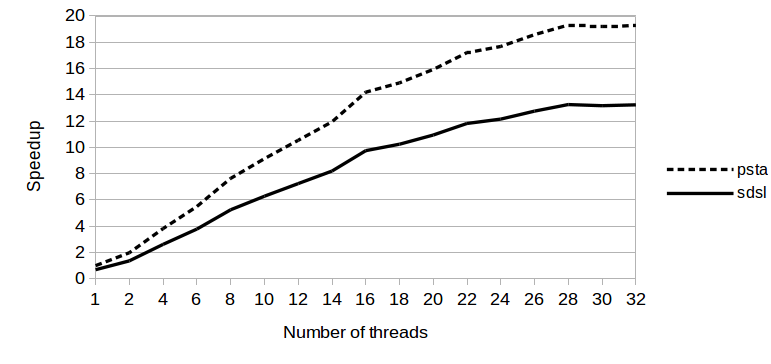
\includegraphics[scale=0.3]{./images/Speedup.png}
  \caption{Speedup of comptree corpus}
  \label{fig:speedup}
\end{figure}

First note that {\tt psta} outperformed {\tt libcds} by an order of magnitude
even on a single core.
As we allowed {\tt psta} to utilize more cores, its advantage over
{\tt libcds} only increased because {\tt libcds} is a purely sequential
program.
{\tt sdsl} was about 1.5 times faster than {\tt psta} on a single core, but
already using two cores {\tt psta} started to be faster than {\tt sdsl}, again
because {\tt sdsl} is a purely sequential program.
The advantage of {\tt sdsl} over {\tt psta} on a single core, in spite of
implementing essentially the same algorithm, can be attributed to (1)
lack of tuning of {\tt psta} and (2) some overhead with running parallel
code on a single core, which {\tt sdsl} avoids by being a purely sequential
program.

Up to 16 cores, the speed-up is almost linear whenever $p$ is a power of $2$,
with an efficiency of 60\%, which is quite good for multicore architectures.
When $p$ is not a power of $2$, speed-up is slightly worse.
The reason is that, when $p$ is a power of $2$, {\tt psta} can assign
exactly one subtree per thread (see Algorithm \ref{algo:PSTA2}),
distributing the work homogeneously across cores and thus not requiring
any work stealing.
When the number of threads is not a power of two, some threads have to process
more than one subtree and other threads process only one, which degrades
performance.  Nevertheless, due to work stealing, no core sits idle for
long and the slight performance degradation is due to the overhead of work
stealing.\Norbert{I made this up.  Does this make sense?  Essentially, the
way it was phrased before doesn't really offer a lot of insight into where
the performance degradation really comes from when the work is not distributed
evenly, and what I wrote here at least matches that we point out that no work
stealing is required when $p = 2^x$.}
For $p = 32$, the efficiency of {\tt psta} drops below 50\%.
This is likely because, on our 32-core machine, less than 32 threads can execute
on their own dedicated cores without interfering with OS processes, which can
run on the 32nd core.
When using 32 threads, the threads of our program start to compete with OS
processes for the available cores, which degrades performance.

The general performance degradation beyond 16 threads is most likely due
to the architecture of the machine we ran our experiments on.
The 4 processors on this machine are arranged in a grid
topology~\cite{Drepper2007}.
Up to 8 threads, communication between the threads is limited to a single
processor running these threads, with very little overhead.
Between 8 and 16 threads require the use of two adjacent processors in
the grid, which still keeps communication cost low.
Beyond 16 threads, three or four processors are needed and at least two
of these processors are not adjacent in the grid, which increases the
communication between the threads on these processors noticeably.
\Leo{Review Drepper's explanation of this}.

Since {\tt psta} generates tasks that work on different memory
regions, the generated cache misses \Leo{false sharing is misses} do
not degrade the performance. The same effect is present on
\emph{Domain Decomposition Algorithms}. Although the decomposition of
the {\tt RMMT} was not evident, we could produce a decomposition that
generated a competitive algorithm.\Norbert{I'm not sure what exactly
you're saying here.  Are you saying that, if the threads were working on the
same memory regions, maintaining cache coherence would essentially force
a lot of reads from RAM because pages in cache become invalid due to writes
by other processors, and given that all our threads work on different memory
regions, this issue does not arise?}
	
\begin{table}[ht]
  \centering
  \begin{tabular}{crrrrr}
\hline
    & xml & dna & psd7003 & protein & comptree\\
\hline
 \verb|psta|   &  1.46  &  1.74  & 2.78  &  3.30 & 112.01\\
 \verb|libcds|   &  .42 &  .58 & .77 &  1.08 & 38.25\\
 \verb|sdsl|   &  .95 &  1.31 & 1.73 &  2.41 & 76.40\\
 \hline
\end{tabular}
\caption{Peak memory consumption of the three algorithms on the data sets
  from Table~\ref{tbl:speedup}, measured in MB.}
\label{tbl:memory_consumption}
\end{table}

Table \ref{tbl:memory_consumption} shows memory consumption for the
corpora usid in our experiments.
For {\tt psta}, the consumption of the single-threaded code ($p = 1$)
is shown.
The extra memory needed for thread scheduling when $p > 1$ was negligible.
To measure memory consumption, we
monitored how much memory was allocated with \texttt{malloc} and
released with \texttt{free} at execution time and recorded the peak
consumption.
We only measured memory allocated during construction of the data structure,
which does not include  the memory allocated to store the parenthesis sequence.
Even though {\tt psta} consumes more memory than both {\tt libcds} and
{\tt sdsl}, the difference between {\tt psta} and {\tt sdsl} is a factor of
less than two.
The difference between {\tt psta} and {\tt libcds} is no more than a factor of
four and is outweighed by the substantially worse performance of {\tt libcds},
even compared to the single-threaded version of {\tt psta}.
More importantly, a memory consumption of 112MB for processing a 1-billion-node
tree amounts to less than one bit per node and, so {\tt psta} can be considered
very space-efficient.

\footnotetext[\value{pizzachili}]{\url{http://pizzachili.dcc.uchile.cl}}
\footnotetext[\value{xmldata}]{\url{http://www.cs.washington.edu/research/xmldatasets}}

Part of the higher memory consumption of {\tt psta} compared to {\tt libcds}
and {\tt sdsl} stems from the allocation of
$e^{\prime}$, $m^{\prime}$, $M^{\prime}$ and $n^{\prime}$ arrays to store the
partial excess values in the algorithm.
Storing these values is a key factor that helps {\tt psta} to achieve very
good performance.
Our implementation allocates 16 bits per excess value in these arrays.
It would be possible to use a simplification
of Algorithm \ref{algo:PSTA1} to calculate the depth $d$ of the input
sequence (the maximum excess value) and then allocate only $\lg d$ bits per
excess value to reduce the space overhead of storing these areas and improve
performance further by reducing the memory bandwidth required to read and write
these arrays.


%%%%%%%%%%%%%%%%%%%%%%
%%%%% CONCLUSION %%%%%
%%%%%%%%%%%%%%%%%%%%%%

\section{Conclusion and Future Work}
\label{sec:conclusion}
In this work we shown that it is possible to improve the construction time of succinct
trees, exploiting current multicore architectures. We introduce a practical algorithm that
achieves $O(\frac{n}{p}+\lg p)$ construction time, to a tree with $n$ nodes and $p$
threads, while supports a rich set of navigational operations in $O(\lg n)$ time. This
practical algorithm was tested against state-of-the-art libraries, reaching good speedup.
We also proposed other algorithm to a more complex succinct tree representation, with
$O(\frac{n\lg p}{p})$ construction time, which supports navegational operations in
constant time. Since our algorithms need, as input, a tree stored as a parentheses
sequence, we presented an algorithm to compute such parentheses sequence in parallel in
$O(\frac{n}{p}+\lg p)$ time.

In this paper we focused on static representation of succinct trees. However, our results
may be the base to the parallel construction of dynamic succinct trees, as the dynamic
succinct trees of \cite{Navarro:2014:FFS:2620785.2601073}. Also, it would be interesting
to study how to extend our results to succinct representation of \emph{labeled} trees. We
shall explore the extension of our results to the parallel construction other succinct
data structures that use succinct trees representations as part of their representations.
Such is the case of succinct planar graphs. Note that we can use the results of
\cite{Fuentes2014} to parallelize batches of navigational operations, reaching a good
pratical speedup. Since that the \emph{range min-max tree}, that our algorithms construct,
is a complete tree, the strategy underlying our algorithms can be applied to construct
general complete trees in parallel.

We believe that exploit current multicore architectures to improve the overall performance
of succinct data structures is a interesting research line. Taking the features of
succinct data structures and the processing power of multicore architectures allows to
design practical data structures with competitive querying time, efficient space usage and
fast/scalable construction time.

\section*{Acknowledgements}

We would like to thank Diego Arroyuelo for discussions about the
implementation of succinct trees, Roberto As\'{i}n for letting us use
his machines to run our experiments, and finally Rodrigo C\'{a}novas
for helping us with reusing their data in
\cite{Navarro:2014:FFS:2620785.2601073}.

\bibliographystyle{splncs03}
\bibliography{sigproc}

\end{document}

